\documentclass[12pt,a4paper]{article}

\usepackage[a4paper,text={16.5cm,25.2cm},centering]{geometry}
\usepackage{lmodern}
\usepackage{amssymb,amsmath}
\usepackage{bm}
\usepackage{graphicx}
\usepackage{microtype}
\usepackage{hyperref}
\usepackage{mhchem}
\setlength{\parindent}{0pt}
\setlength{\parskip}{1.2ex}

\hypersetup
       {   pdfauthor = {  },
           pdftitle={  },
           colorlinks=TRUE,
           linkcolor=black,
           citecolor=blue,
           urlcolor=blue
       }




\usepackage{upquote}
\usepackage{listings}
\usepackage{xcolor}
\lstset{
    basicstyle=\ttfamily\footnotesize,
    upquote=true,
    breaklines=true,
    breakindent=0pt,
    keepspaces=true,
    showspaces=false,
    columns=fullflexible,
    showtabs=false,
    showstringspaces=false,
    escapeinside={(*@}{@*)},
    extendedchars=true,
}
\newcommand{\HLJLt}[1]{#1}
\newcommand{\HLJLw}[1]{#1}
\newcommand{\HLJLe}[1]{#1}
\newcommand{\HLJLeB}[1]{#1}
\newcommand{\HLJLo}[1]{#1}
\newcommand{\HLJLk}[1]{\textcolor[RGB]{148,91,176}{\textbf{#1}}}
\newcommand{\HLJLkc}[1]{\textcolor[RGB]{59,151,46}{\textit{#1}}}
\newcommand{\HLJLkd}[1]{\textcolor[RGB]{214,102,97}{\textit{#1}}}
\newcommand{\HLJLkn}[1]{\textcolor[RGB]{148,91,176}{\textbf{#1}}}
\newcommand{\HLJLkp}[1]{\textcolor[RGB]{148,91,176}{\textbf{#1}}}
\newcommand{\HLJLkr}[1]{\textcolor[RGB]{148,91,176}{\textbf{#1}}}
\newcommand{\HLJLkt}[1]{\textcolor[RGB]{148,91,176}{\textbf{#1}}}
\newcommand{\HLJLn}[1]{#1}
\newcommand{\HLJLna}[1]{#1}
\newcommand{\HLJLnb}[1]{#1}
\newcommand{\HLJLnbp}[1]{#1}
\newcommand{\HLJLnc}[1]{#1}
\newcommand{\HLJLncB}[1]{#1}
\newcommand{\HLJLnd}[1]{\textcolor[RGB]{214,102,97}{#1}}
\newcommand{\HLJLne}[1]{#1}
\newcommand{\HLJLneB}[1]{#1}
\newcommand{\HLJLnf}[1]{\textcolor[RGB]{66,102,213}{#1}}
\newcommand{\HLJLnfm}[1]{\textcolor[RGB]{66,102,213}{#1}}
\newcommand{\HLJLnp}[1]{#1}
\newcommand{\HLJLnl}[1]{#1}
\newcommand{\HLJLnn}[1]{#1}
\newcommand{\HLJLno}[1]{#1}
\newcommand{\HLJLnt}[1]{#1}
\newcommand{\HLJLnv}[1]{#1}
\newcommand{\HLJLnvc}[1]{#1}
\newcommand{\HLJLnvg}[1]{#1}
\newcommand{\HLJLnvi}[1]{#1}
\newcommand{\HLJLnvm}[1]{#1}
\newcommand{\HLJLl}[1]{#1}
\newcommand{\HLJLld}[1]{\textcolor[RGB]{148,91,176}{\textit{#1}}}
\newcommand{\HLJLs}[1]{\textcolor[RGB]{201,61,57}{#1}}
\newcommand{\HLJLsa}[1]{\textcolor[RGB]{201,61,57}{#1}}
\newcommand{\HLJLsb}[1]{\textcolor[RGB]{201,61,57}{#1}}
\newcommand{\HLJLsc}[1]{\textcolor[RGB]{201,61,57}{#1}}
\newcommand{\HLJLsd}[1]{\textcolor[RGB]{201,61,57}{#1}}
\newcommand{\HLJLsdB}[1]{\textcolor[RGB]{201,61,57}{#1}}
\newcommand{\HLJLsdC}[1]{\textcolor[RGB]{201,61,57}{#1}}
\newcommand{\HLJLse}[1]{\textcolor[RGB]{59,151,46}{#1}}
\newcommand{\HLJLsh}[1]{\textcolor[RGB]{201,61,57}{#1}}
\newcommand{\HLJLsi}[1]{#1}
\newcommand{\HLJLso}[1]{\textcolor[RGB]{201,61,57}{#1}}
\newcommand{\HLJLsr}[1]{\textcolor[RGB]{201,61,57}{#1}}
\newcommand{\HLJLss}[1]{\textcolor[RGB]{201,61,57}{#1}}
\newcommand{\HLJLssB}[1]{\textcolor[RGB]{201,61,57}{#1}}
\newcommand{\HLJLnB}[1]{\textcolor[RGB]{59,151,46}{#1}}
\newcommand{\HLJLnbB}[1]{\textcolor[RGB]{59,151,46}{#1}}
\newcommand{\HLJLnfB}[1]{\textcolor[RGB]{59,151,46}{#1}}
\newcommand{\HLJLnh}[1]{\textcolor[RGB]{59,151,46}{#1}}
\newcommand{\HLJLni}[1]{\textcolor[RGB]{59,151,46}{#1}}
\newcommand{\HLJLnil}[1]{\textcolor[RGB]{59,151,46}{#1}}
\newcommand{\HLJLnoB}[1]{\textcolor[RGB]{59,151,46}{#1}}
\newcommand{\HLJLoB}[1]{\textcolor[RGB]{102,102,102}{\textbf{#1}}}
\newcommand{\HLJLow}[1]{\textcolor[RGB]{102,102,102}{\textbf{#1}}}
\newcommand{\HLJLp}[1]{#1}
\newcommand{\HLJLc}[1]{\textcolor[RGB]{153,153,119}{\textit{#1}}}
\newcommand{\HLJLch}[1]{\textcolor[RGB]{153,153,119}{\textit{#1}}}
\newcommand{\HLJLcm}[1]{\textcolor[RGB]{153,153,119}{\textit{#1}}}
\newcommand{\HLJLcp}[1]{\textcolor[RGB]{153,153,119}{\textit{#1}}}
\newcommand{\HLJLcpB}[1]{\textcolor[RGB]{153,153,119}{\textit{#1}}}
\newcommand{\HLJLcs}[1]{\textcolor[RGB]{153,153,119}{\textit{#1}}}
\newcommand{\HLJLcsB}[1]{\textcolor[RGB]{153,153,119}{\textit{#1}}}
\newcommand{\HLJLg}[1]{#1}
\newcommand{\HLJLgd}[1]{#1}
\newcommand{\HLJLge}[1]{#1}
\newcommand{\HLJLgeB}[1]{#1}
\newcommand{\HLJLgh}[1]{#1}
\newcommand{\HLJLgi}[1]{#1}
\newcommand{\HLJLgo}[1]{#1}
\newcommand{\HLJLgp}[1]{#1}
\newcommand{\HLJLgs}[1]{#1}
\newcommand{\HLJLgsB}[1]{#1}
\newcommand{\HLJLgt}[1]{#1}


\begin{document}



\section{Shared memory}
In this example we will explore shared memory. We will use array reversal and matrix transpose as examples.

\textbf{Shared memory} is the memory in a SM(symmetric multiprocessor) which is accessable to all threads running on the SM. It is much faster than global memory much closer. The amount of shared memory available depends on the compute capability of the GPU. Increasing the amount of shared memory reduces occupancy.

\texttt{syncthreads()} is a function which adds a \href{https://en.wikipedia.org/wiki/Barrier_(computer_science)}{barrier} for all threads in a thread block. While all threads in a block execute concurrently, physically only a subset of these are running with true parallelism. A barrier ensures that all threads which belong to it stall until all have reached the barrier. This is commonly used as a synchronization mechanism to eliminate race conditions.

\subsubsection{Array Reversal}
Our job is to reverse an array, i.e $[1, 2, 3] \rightarrow [3, 2, 1]$.


\begin{lstlisting}
(*@\HLJLk{using}@*) (*@\HLJLn{CUDA}@*)(*@\HLJLp{,}@*) (*@\HLJLn{BenchmarkTools}@*)

(*@\HLJLk{function}@*) (*@\HLJLnf{reverse}@*)(*@\HLJLp{(}@*)(*@\HLJLn{input}@*)(*@\HLJLp{,}@*) (*@\HLJLn{output}@*) (*@\HLJLoB{=}@*) (*@\HLJLnf{similar}@*)(*@\HLJLp{(}@*)(*@\HLJLn{input}@*)(*@\HLJLp{))}@*)
    (*@\HLJLn{len}@*) (*@\HLJLoB{=}@*) (*@\HLJLnf{length}@*)(*@\HLJLp{(}@*)(*@\HLJLn{input}@*)(*@\HLJLp{)}@*)
    (*@\HLJLk{for}@*) (*@\HLJLn{i}@*) (*@\HLJLoB{=}@*) (*@\HLJLni{1}@*)(*@\HLJLoB{:}@*)(*@\HLJLnf{cld}@*)(*@\HLJLp{(}@*)(*@\HLJLn{len}@*)(*@\HLJLp{,}@*)(*@\HLJLni{2}@*)(*@\HLJLp{)}@*)
        (*@\HLJLn{output}@*)(*@\HLJLp{[}@*)(*@\HLJLn{i}@*)(*@\HLJLp{],}@*) (*@\HLJLn{output}@*)(*@\HLJLp{[}@*)(*@\HLJLn{len}@*) (*@\HLJLoB{-}@*) (*@\HLJLn{i}@*) (*@\HLJLoB{+}@*) (*@\HLJLni{1}@*)(*@\HLJLp{]}@*) (*@\HLJLoB{=}@*) (*@\HLJLn{input}@*)(*@\HLJLp{[}@*)(*@\HLJLn{len}@*) (*@\HLJLoB{-}@*) (*@\HLJLn{i}@*) (*@\HLJLoB{+}@*) (*@\HLJLni{1}@*)(*@\HLJLp{],}@*) (*@\HLJLn{input}@*)(*@\HLJLp{[}@*)(*@\HLJLn{i}@*)(*@\HLJLp{]}@*)
    (*@\HLJLk{end}@*)
    (*@\HLJLn{output}@*)
(*@\HLJLk{end}@*)
\end{lstlisting}

\begin{lstlisting}
reverse (generic function with 2 methods)
\end{lstlisting}


\begin{lstlisting}
(*@\HLJLnf{reverse}@*)(*@\HLJLp{([}@*)(*@\HLJLni{1}@*)(*@\HLJLp{,}@*) (*@\HLJLni{2}@*)(*@\HLJLp{,}@*) (*@\HLJLni{3}@*)(*@\HLJLp{,}@*) (*@\HLJLni{4}@*)(*@\HLJLp{,}@*) (*@\HLJLni{5}@*)(*@\HLJLp{])}@*)
\end{lstlisting}

\begin{lstlisting}
5-element Array(*@{{\{}}@*)Int64,1(*@{{\}}}@*):
 5
 4
 3
 2
 1
\end{lstlisting}


\begin{lstlisting}
(*@\HLJLk{function}@*) (*@\HLJLnf{gpu{\_}reverse}@*)(*@\HLJLp{(}@*)(*@\HLJLn{input}@*)(*@\HLJLp{,}@*) (*@\HLJLn{output}@*)(*@\HLJLp{)}@*)
    (*@\HLJLn{tid}@*) (*@\HLJLoB{=}@*) (*@\HLJLnf{threadIdx}@*)(*@\HLJLp{()}@*)(*@\HLJLoB{.}@*)(*@\HLJLn{x}@*)
    (*@\HLJLn{len}@*) (*@\HLJLoB{=}@*) (*@\HLJLnf{length}@*)(*@\HLJLp{(}@*)(*@\HLJLn{input}@*)(*@\HLJLp{)}@*)
    (*@\HLJLk{if}@*) (*@\HLJLn{tid}@*) (*@\HLJLoB{<=}@*) (*@\HLJLnf{cld}@*)(*@\HLJLp{(}@*)(*@\HLJLn{len}@*)(*@\HLJLp{,}@*) (*@\HLJLni{2}@*)(*@\HLJLp{)}@*)
        (*@\HLJLn{output}@*)(*@\HLJLp{[}@*)(*@\HLJLn{tid}@*)(*@\HLJLp{],}@*) (*@\HLJLn{output}@*)(*@\HLJLp{[}@*)(*@\HLJLn{len}@*) (*@\HLJLoB{-}@*) (*@\HLJLn{tid}@*) (*@\HLJLoB{+}@*) (*@\HLJLni{1}@*)(*@\HLJLp{]}@*) (*@\HLJLoB{=}@*) (*@\HLJLn{input}@*)(*@\HLJLp{[}@*)(*@\HLJLn{len}@*) (*@\HLJLoB{-}@*) (*@\HLJLn{tid}@*) (*@\HLJLoB{+}@*) (*@\HLJLni{1}@*)(*@\HLJLp{],}@*) (*@\HLJLn{input}@*)(*@\HLJLp{[}@*)(*@\HLJLn{tid}@*)(*@\HLJLp{]}@*)
    (*@\HLJLk{end}@*)
    (*@\HLJLk{return}@*)
(*@\HLJLk{end}@*)
\end{lstlisting}

\begin{lstlisting}
gpu(*@{{\_}}@*)reverse (generic function with 1 method)
\end{lstlisting}


\begin{lstlisting}
(*@\HLJLn{A}@*) (*@\HLJLoB{=}@*) (*@\HLJLnf{CuArray}@*)(*@\HLJLp{(}@*)(*@\HLJLnf{collect}@*)(*@\HLJLp{(}@*)(*@\HLJLni{1}@*)(*@\HLJLoB{:}@*)(*@\HLJLni{5}@*)(*@\HLJLp{))}@*)
(*@\HLJLn{B}@*) (*@\HLJLoB{=}@*) (*@\HLJLnf{similar}@*)(*@\HLJLp{(}@*)(*@\HLJLn{A}@*)(*@\HLJLp{)}@*)
(*@\HLJLnd{@cuda}@*) (*@\HLJLn{blocks}@*)(*@\HLJLoB{=}@*)(*@\HLJLni{1}@*) (*@\HLJLn{threads}@*)(*@\HLJLoB{=}@*)(*@\HLJLnf{length}@*)(*@\HLJLp{(}@*)(*@\HLJLn{A}@*)(*@\HLJLp{)}@*) (*@\HLJLnf{gpu{\_}reverse}@*)(*@\HLJLp{(}@*)(*@\HLJLn{A}@*)(*@\HLJLp{,}@*) (*@\HLJLn{B}@*)(*@\HLJLp{)}@*)
(*@\HLJLn{B}@*)
\end{lstlisting}

\begin{lstlisting}
5-element CUDA.CuArray(*@{{\{}}@*)Int64,1(*@{{\}}}@*):
 5
 4
 3
 2
 1
\end{lstlisting}


There are two ways to declare shared memory: Statically and Dynamically. We declaring it statically when we the need is the same amount for all kernel launches and its known while writing the kernel. In the other case we declare it dynamically and specify while launching with the \texttt{@cuda} macro using the \texttt{shmem} argument.


\begin{lstlisting}
(*@\HLJLoB{?}@*)(*@\HLJLnd{@cuStaticSharedMem}@*)
\end{lstlisting}

\begin{lstlisting}
Error: syntax: invalid identifier name (*@{"{}}@*)?(*@{"{}}@*)
\end{lstlisting}


\begin{lstlisting}
(*@\HLJLk{function}@*) (*@\HLJLnf{gpu{\_}stshmemreverse}@*)(*@\HLJLp{(}@*)(*@\HLJLn{input}@*)(*@\HLJLp{,}@*) (*@\HLJLn{output}@*)(*@\HLJLp{)}@*)
    (*@\HLJLcs{{\#}}@*) (*@\HLJLcs{Maximum}@*) (*@\HLJLcs{size}@*) (*@\HLJLcs{of}@*) (*@\HLJLcs{array}@*) (*@\HLJLcs{is}@*) (*@\HLJLcs{64}@*)
    (*@\HLJLn{shmem}@*) (*@\HLJLoB{=}@*) (*@\HLJLnd{@cuStaticSharedMem}@*)(*@\HLJLp{(}@*)(*@\HLJLnf{eltype}@*)(*@\HLJLp{(}@*)(*@\HLJLn{output}@*)(*@\HLJLp{),}@*) (*@\HLJLni{64}@*)(*@\HLJLp{)}@*)
    (*@\HLJLn{tid}@*) (*@\HLJLoB{=}@*) (*@\HLJLnf{threadIdx}@*)(*@\HLJLp{()}@*)(*@\HLJLoB{.}@*)(*@\HLJLn{x}@*)
    (*@\HLJLn{len}@*) (*@\HLJLoB{=}@*) (*@\HLJLnf{length}@*)(*@\HLJLp{(}@*)(*@\HLJLn{input}@*)(*@\HLJLp{)}@*)
    (*@\HLJLn{shmem}@*)(*@\HLJLp{[}@*)(*@\HLJLn{tid}@*)(*@\HLJLp{]}@*) (*@\HLJLoB{=}@*) (*@\HLJLn{input}@*)(*@\HLJLp{[}@*)(*@\HLJLn{len}@*) (*@\HLJLoB{-}@*) (*@\HLJLn{tid}@*) (*@\HLJLoB{+}@*) (*@\HLJLni{1}@*)(*@\HLJLp{]}@*)
    (*@\HLJLn{output}@*)(*@\HLJLp{[}@*)(*@\HLJLn{tid}@*)(*@\HLJLp{]}@*) (*@\HLJLoB{=}@*) (*@\HLJLn{shmem}@*)(*@\HLJLp{[}@*)(*@\HLJLn{tid}@*)(*@\HLJLp{]}@*)
    (*@\HLJLk{return}@*)
(*@\HLJLk{end}@*)
\end{lstlisting}

\begin{lstlisting}
gpu(*@{{\_}}@*)stshmemreverse (generic function with 1 method)
\end{lstlisting}


\begin{lstlisting}
(*@\HLJLn{A}@*) (*@\HLJLoB{=}@*) (*@\HLJLnf{CuArray}@*)(*@\HLJLp{(}@*)(*@\HLJLnf{collect}@*)(*@\HLJLp{(}@*)(*@\HLJLni{1}@*)(*@\HLJLoB{:}@*)(*@\HLJLni{32}@*)(*@\HLJLp{))}@*)
(*@\HLJLn{B}@*) (*@\HLJLoB{=}@*) (*@\HLJLnf{similar}@*)(*@\HLJLp{(}@*)(*@\HLJLn{A}@*)(*@\HLJLp{)}@*)
(*@\HLJLnd{@cuda}@*) (*@\HLJLn{blocks}@*)(*@\HLJLoB{=}@*)(*@\HLJLni{1}@*) (*@\HLJLn{threads}@*)(*@\HLJLoB{=}@*)(*@\HLJLnf{length}@*)(*@\HLJLp{(}@*)(*@\HLJLn{A}@*)(*@\HLJLp{)}@*) (*@\HLJLnf{gpu{\_}stshmemreverse}@*)(*@\HLJLp{(}@*)(*@\HLJLn{A}@*)(*@\HLJLp{,}@*) (*@\HLJLn{B}@*)(*@\HLJLp{)}@*)
(*@\HLJLnf{print}@*)(*@\HLJLp{(}@*)(*@\HLJLn{B}@*)(*@\HLJLp{)}@*)
\end{lstlisting}

\begin{lstlisting}
[32, 31, 30, 29, 28, 27, 26, 25, 24, 23, 22, 21, 20, 19, 18, 17, 16, 15, 14
, 13, 12, 11, 10, 9, 8, 7, 6, 5, 4, 3, 2, 1]
\end{lstlisting}


When the amount of shared memory required isn't known while writing the kernel overallocating is not a good idea because that may potentially reduce our occupancy. As an SM's resource usage increases it's occupancy goes down. Hence, it's best to use dynamically allocated memory when memory usage can only be known at launch time.


\begin{lstlisting}
(*@\HLJLoB{?}@*)(*@\HLJLnd{@cuDynamicSharedMem}@*)
\end{lstlisting}

\begin{lstlisting}
Error: syntax: invalid identifier name (*@{"{}}@*)?(*@{"{}}@*)
\end{lstlisting}


\begin{lstlisting}
(*@\HLJLk{function}@*) (*@\HLJLnf{gpu{\_}dyshmemreverse}@*)(*@\HLJLp{(}@*)(*@\HLJLn{input}@*)(*@\HLJLp{,}@*) (*@\HLJLn{output}@*)(*@\HLJLp{)}@*)
    (*@\HLJLn{shmem}@*) (*@\HLJLoB{=}@*) (*@\HLJLnd{@cuDynamicSharedMem}@*)(*@\HLJLp{(}@*)(*@\HLJLnf{eltype}@*)(*@\HLJLp{(}@*)(*@\HLJLn{output}@*)(*@\HLJLp{),}@*) (*@\HLJLp{(}@*)(*@\HLJLnf{length}@*)(*@\HLJLp{(}@*)(*@\HLJLn{output}@*)(*@\HLJLp{),))}@*)
    (*@\HLJLn{tid}@*) (*@\HLJLoB{=}@*) (*@\HLJLnf{threadIdx}@*)(*@\HLJLp{()}@*)(*@\HLJLoB{.}@*)(*@\HLJLn{x}@*)
    (*@\HLJLn{len}@*) (*@\HLJLoB{=}@*) (*@\HLJLnf{length}@*)(*@\HLJLp{(}@*)(*@\HLJLn{input}@*)(*@\HLJLp{)}@*)
    (*@\HLJLn{shmem}@*)(*@\HLJLp{[}@*)(*@\HLJLn{tid}@*)(*@\HLJLp{]}@*) (*@\HLJLoB{=}@*) (*@\HLJLn{input}@*)(*@\HLJLp{[}@*)(*@\HLJLn{len}@*) (*@\HLJLoB{-}@*) (*@\HLJLn{tid}@*) (*@\HLJLoB{+}@*) (*@\HLJLni{1}@*)(*@\HLJLp{]}@*)
    (*@\HLJLn{output}@*)(*@\HLJLp{[}@*)(*@\HLJLn{tid}@*)(*@\HLJLp{]}@*) (*@\HLJLoB{=}@*) (*@\HLJLn{shmem}@*)(*@\HLJLp{[}@*)(*@\HLJLn{tid}@*)(*@\HLJLp{]}@*)
    (*@\HLJLk{return}@*)
(*@\HLJLk{end}@*)
\end{lstlisting}

\begin{lstlisting}
gpu(*@{{\_}}@*)dyshmemreverse (generic function with 1 method)
\end{lstlisting}


\begin{lstlisting}
(*@\HLJLn{C}@*) (*@\HLJLoB{=}@*) (*@\HLJLnf{CuArray}@*)(*@\HLJLp{(}@*)(*@\HLJLnf{collect}@*)(*@\HLJLp{(}@*)(*@\HLJLni{1}@*)(*@\HLJLoB{:}@*)(*@\HLJLni{32}@*)(*@\HLJLp{))}@*)
(*@\HLJLn{D}@*) (*@\HLJLoB{=}@*) (*@\HLJLnf{similar}@*)(*@\HLJLp{(}@*)(*@\HLJLn{C}@*)(*@\HLJLp{)}@*)
(*@\HLJLnd{@cuda}@*) (*@\HLJLn{blocks}@*)(*@\HLJLoB{=}@*)(*@\HLJLni{1}@*) (*@\HLJLn{threads}@*)(*@\HLJLoB{=}@*)(*@\HLJLnf{length}@*)(*@\HLJLp{(}@*)(*@\HLJLn{C}@*)(*@\HLJLp{)}@*) (*@\HLJLn{shmem}@*)(*@\HLJLoB{=}@*)(*@\HLJLnf{length}@*)(*@\HLJLp{(}@*)(*@\HLJLn{C}@*)(*@\HLJLp{)}@*) (*@\HLJLnf{gpu{\_}dyshmemreverse}@*)(*@\HLJLp{(}@*)(*@\HLJLn{C}@*)(*@\HLJLp{,}@*) (*@\HLJLn{D}@*)(*@\HLJLp{)}@*)
(*@\HLJLnf{print}@*)(*@\HLJLp{(}@*)(*@\HLJLn{D}@*)(*@\HLJLp{)}@*)
\end{lstlisting}

\begin{lstlisting}
[32, 31, 30, 29, 28, 27, 26, 25, 24, 23, 22, 21, 20, 19, 18, 17, 16, 15, 14
, 13, 12, 11, 10, 9, 8, 7, 6, 5, 4, 3, 2, 1]
\end{lstlisting}


\subsection{Matrix Transpose}
Matrix transpose is an operation which flips a matrix along its main diagonal.

\begin{figure}
\centering
\includegraphics{https://upload.wikimedia.org/wikipedia/commons/e/e4/Matrix_transpose.gif =250x250}
\caption{Matrix Transpose animation}
\end{figure}


\begin{figure}
\centering
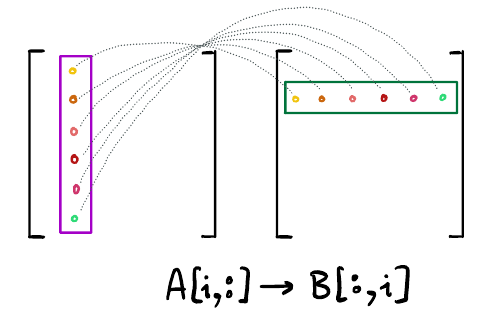
\includegraphics{./assets/transpose.png}
\caption{transpose}
\end{figure}


This section is inspired by Mark Harris' blog post on the same topic. \href{https://developer.nvidia.com/blog/efficient-matrix-transpose-cuda-cc/}{Link}


\begin{lstlisting}
(*@\HLJLn{A}@*) (*@\HLJLoB{=}@*) (*@\HLJLnf{reshape}@*)(*@\HLJLp{(}@*)(*@\HLJLni{1}@*)(*@\HLJLoB{:}@*)(*@\HLJLni{9}@*)(*@\HLJLp{,}@*) (*@\HLJLp{(}@*)(*@\HLJLni{3}@*)(*@\HLJLp{,}@*) (*@\HLJLni{3}@*)(*@\HLJLp{))}@*)
\end{lstlisting}

\begin{lstlisting}
3(*@\ensuremath{\times}@*)3 reshape(::UnitRange(*@{{\{}}@*)Int64(*@{{\}}}@*), 3, 3) with eltype Int64:
 1  4  7
 2  5  8
 3  6  9
\end{lstlisting}


\begin{lstlisting}
(*@\HLJLn{A}@*)(*@\HLJLoB{{\textquotesingle}}@*)
\end{lstlisting}

\begin{lstlisting}
3(*@\ensuremath{\times}@*)3 LinearAlgebra.Adjoint(*@{{\{}}@*)Int64,Base.ReshapedArray(*@{{\{}}@*)Int64,2,UnitRange(*@{{\{}}@*)Int64(*@{{\}}}@*)
,Tuple(*@{{\{}}@*)(*@{{\}}}@*)(*@{{\}}}@*)(*@{{\}}}@*):
 1  2  3
 4  5  6
 7  8  9
\end{lstlisting}


\begin{lstlisting}
(*@\HLJLn{A}@*)(*@\HLJLoB{{\textquotesingle}{\textquotesingle}}@*) (*@\HLJLcs{{\#}}@*) (*@\HLJLcs{(A{\textquotesingle}){\textquotesingle}}@*)
\end{lstlisting}

\begin{lstlisting}
3(*@\ensuremath{\times}@*)3 reshape(::UnitRange(*@{{\{}}@*)Int64(*@{{\}}}@*), 3, 3) with eltype Int64:
 1  4  7
 2  5  8
 3  6  9
\end{lstlisting}


Ignore the types that Julia returns. \texttt{LinearAlgebra.Adjoint} is a wrapper that uses \href{https://en.wikipedia.org/wiki/Lazy_evaluation}{lazy evaluation} to compute the result as required.


\begin{lstlisting}
(*@\HLJLcs{{\#}}@*) (*@\HLJLcs{CPU}@*) (*@\HLJLcs{implementation}@*)
(*@\HLJLk{function}@*) (*@\HLJLnf{cpu{\_}transpose}@*)(*@\HLJLp{(}@*)(*@\HLJLn{input}@*)(*@\HLJLp{,}@*) (*@\HLJLn{output}@*) (*@\HLJLoB{=}@*) (*@\HLJLnf{similar}@*)(*@\HLJLp{(}@*)(*@\HLJLn{input}@*)(*@\HLJLp{,}@*) (*@\HLJLp{(}@*)(*@\HLJLnf{size}@*)(*@\HLJLp{(}@*)(*@\HLJLn{input}@*)(*@\HLJLp{,}@*) (*@\HLJLni{2}@*)(*@\HLJLp{),}@*) (*@\HLJLnf{size}@*)(*@\HLJLp{(}@*)(*@\HLJLn{input}@*)(*@\HLJLp{,}@*) (*@\HLJLni{1}@*)(*@\HLJLp{))))}@*)
    (*@\HLJLcs{{\#}}@*) (*@\HLJLcs{the}@*) (*@\HLJLcs{dimensions}@*) (*@\HLJLcs{of}@*) (*@\HLJLcs{the}@*) (*@\HLJLcs{resultant}@*) (*@\HLJLcs{matrix}@*) (*@\HLJLcs{are}@*) (*@\HLJLcs{reversed}@*)
    (*@\HLJLk{for}@*) (*@\HLJLn{index}@*) (*@\HLJLoB{=}@*) (*@\HLJLnf{CartesianIndices}@*)(*@\HLJLp{(}@*)(*@\HLJLn{input}@*)(*@\HLJLp{)}@*)
            (*@\HLJLn{output}@*)(*@\HLJLp{[}@*)(*@\HLJLn{index}@*)(*@\HLJLp{[}@*)(*@\HLJLni{2}@*)(*@\HLJLp{],}@*) (*@\HLJLn{index}@*)(*@\HLJLp{[}@*)(*@\HLJLni{1}@*)(*@\HLJLp{]]}@*) (*@\HLJLoB{=}@*) (*@\HLJLn{input}@*)(*@\HLJLp{[}@*)(*@\HLJLn{index}@*)(*@\HLJLp{]}@*)
    (*@\HLJLk{end}@*)
    (*@\HLJLn{output}@*)
(*@\HLJLk{end}@*)
\end{lstlisting}

\begin{lstlisting}
cpu(*@{{\_}}@*)transpose (generic function with 2 methods)
\end{lstlisting}


\begin{lstlisting}
(*@\HLJLn{A}@*) (*@\HLJLoB{=}@*) (*@\HLJLnf{reshape}@*)(*@\HLJLp{(}@*)(*@\HLJLni{1}@*)(*@\HLJLoB{:}@*)(*@\HLJLni{20}@*)(*@\HLJLp{,}@*) (*@\HLJLp{(}@*)(*@\HLJLni{4}@*)(*@\HLJLp{,}@*) (*@\HLJLni{5}@*)(*@\HLJLp{))}@*)
\end{lstlisting}

\begin{lstlisting}
4(*@\ensuremath{\times}@*)5 reshape(::UnitRange(*@{{\{}}@*)Int64(*@{{\}}}@*), 4, 5) with eltype Int64:
 1  5   9  13  17
 2  6  10  14  18
 3  7  11  15  19
 4  8  12  16  20
\end{lstlisting}


\begin{lstlisting}
(*@\HLJLnf{cpu{\_}transpose}@*)(*@\HLJLp{(}@*)(*@\HLJLn{A}@*)(*@\HLJLp{)}@*)
\end{lstlisting}

\begin{lstlisting}
5(*@\ensuremath{\times}@*)4 Array(*@{{\{}}@*)Int64,2(*@{{\}}}@*):
  1   2   3   4
  5   6   7   8
  9  10  11  12
 13  14  15  16
 17  18  19  20
\end{lstlisting}


Before we begin working on the GPU consider the following code.


\begin{lstlisting}
(*@\HLJLn{A}@*) (*@\HLJLoB{=}@*) (*@\HLJLnf{CuArray}@*)(*@\HLJLp{(}@*)(*@\HLJLnf{reshape}@*)(*@\HLJLp{(}@*)(*@\HLJLnfB{1.}@*)(*@\HLJLoB{:}@*)(*@\HLJLni{9}@*)(*@\HLJLp{,}@*) (*@\HLJLp{(}@*)(*@\HLJLni{3}@*)(*@\HLJLp{,}@*) (*@\HLJLni{3}@*)(*@\HLJLp{)))}@*)

(*@\HLJLnf{println}@*)(*@\HLJLp{(}@*)(*@\HLJLs{"{}A}@*) (*@\HLJLs{=>}@*) (*@\HLJLs{"{}}@*)(*@\HLJLp{,}@*) (*@\HLJLnf{pointer}@*)(*@\HLJLp{(}@*)(*@\HLJLn{A}@*)(*@\HLJLp{))}@*)
(*@\HLJLn{CUDA}@*)(*@\HLJLoB{.}@*)(*@\HLJLnd{@allowscalar}@*) (*@\HLJLk{begin}@*)
    (*@\HLJLk{for}@*) (*@\HLJLn{i}@*) (*@\HLJLkp{in}@*) (*@\HLJLnf{eachindex}@*)(*@\HLJLp{(}@*)(*@\HLJLn{A}@*)(*@\HLJLp{)}@*)
        (*@\HLJLnf{println}@*)(*@\HLJLp{(}@*)(*@\HLJLn{i}@*)(*@\HLJLp{,}@*) (*@\HLJLs{"{}}@*) (*@\HLJLs{"{}}@*)(*@\HLJLp{,}@*) (*@\HLJLn{A}@*)(*@\HLJLp{[}@*)(*@\HLJLn{i}@*)(*@\HLJLp{],}@*) (*@\HLJLs{"{}}@*) (*@\HLJLs{"{}}@*)(*@\HLJLp{,}@*) (*@\HLJLnf{pointer}@*)(*@\HLJLp{(}@*)(*@\HLJLn{A}@*)(*@\HLJLp{,}@*) (*@\HLJLn{i}@*)(*@\HLJLp{))}@*)
    (*@\HLJLk{end}@*)
(*@\HLJLk{end}@*)
\end{lstlisting}

\begin{lstlisting}
A => CUDA.CuPtr(*@{{\{}}@*)Float64(*@{{\}}}@*)(0x00007fbce2831800)
1 1.0 CUDA.CuPtr(*@{{\{}}@*)Float64(*@{{\}}}@*)(0x00007fbce2831800)
2 2.0 CUDA.CuPtr(*@{{\{}}@*)Float64(*@{{\}}}@*)(0x00007fbce2831808)
3 3.0 CUDA.CuPtr(*@{{\{}}@*)Float64(*@{{\}}}@*)(0x00007fbce2831810)
4 4.0 CUDA.CuPtr(*@{{\{}}@*)Float64(*@{{\}}}@*)(0x00007fbce2831818)
5 5.0 CUDA.CuPtr(*@{{\{}}@*)Float64(*@{{\}}}@*)(0x00007fbce2831820)
6 6.0 CUDA.CuPtr(*@{{\{}}@*)Float64(*@{{\}}}@*)(0x00007fbce2831828)
7 7.0 CUDA.CuPtr(*@{{\{}}@*)Float64(*@{{\}}}@*)(0x00007fbce2831830)
8 8.0 CUDA.CuPtr(*@{{\{}}@*)Float64(*@{{\}}}@*)(0x00007fbce2831838)
9 9.0 CUDA.CuPtr(*@{{\{}}@*)Float64(*@{{\}}}@*)(0x00007fbce2831840)
\end{lstlisting}


Notice how consecutive elements are in the same column rather than the same row. This is because Julia stores its multidimensional arrays in a column major order like Fortran. In contrast to C/C++ which are row-major languages. The reason for making Julia's arrays column major is because a lot of linear algebra libraries are column major to begin with (https://discourse.julialang.org/t/why-column-major/24374/3).


\begin{lstlisting}
(*@\HLJLcs{{\#}}@*) (*@\HLJLcs{To}@*) (*@\HLJLcs{index}@*) (*@\HLJLcs{our}@*) (*@\HLJLcs{2-D}@*) (*@\HLJLcs{array}@*) (*@\HLJLcs{we}@*) (*@\HLJLcs{will}@*) (*@\HLJLcs{split}@*) (*@\HLJLcs{the}@*) (*@\HLJLcs{input}@*) (*@\HLJLcs{into}@*) (*@\HLJLcs{tiles}@*) (*@\HLJLcs{of}@*) (*@\HLJLcs{32x32}@*) (*@\HLJLcs{elements.}@*) 
(*@\HLJLcs{{\#}}@*) (*@\HLJLcs{Each}@*) (*@\HLJLcs{thread}@*) (*@\HLJLcs{block}@*) (*@\HLJLcs{will}@*) (*@\HLJLcs{launch}@*) (*@\HLJLcs{with}@*) (*@\HLJLcs{32x8}@*) (*@\HLJLcs{=}@*) (*@\HLJLcs{256}@*) (*@\HLJLcs{threads}@*) 
(*@\HLJLcs{{\#}}@*) (*@\HLJLcs{Each}@*) (*@\HLJLcs{thread}@*) (*@\HLJLcs{will}@*) (*@\HLJLcs{work}@*) (*@\HLJLcs{on}@*) (*@\HLJLcs{4}@*) (*@\HLJLcs{elements.}@*)
(*@\HLJLkd{const}@*) (*@\HLJLn{TILE{\_}DIM}@*) (*@\HLJLoB{=}@*) (*@\HLJLni{32}@*)

(*@\HLJLk{function}@*) (*@\HLJLnf{gpu{\_}transpose{\_}kernel}@*)(*@\HLJLp{(}@*)(*@\HLJLn{input}@*)(*@\HLJLp{,}@*) (*@\HLJLn{output}@*)(*@\HLJLp{)}@*)
    (*@\HLJLn{tile{\_}index}@*) (*@\HLJLoB{=}@*) (*@\HLJLp{((}@*)(*@\HLJLnf{blockIdx}@*)(*@\HLJLp{()}@*)(*@\HLJLoB{.}@*)(*@\HLJLn{y}@*)(*@\HLJLp{,}@*) (*@\HLJLnf{blockIdx}@*)(*@\HLJLp{()}@*)(*@\HLJLoB{.}@*)(*@\HLJLn{x}@*)(*@\HLJLp{)}@*) (*@\HLJLoB{.-}@*) (*@\HLJLni{1}@*)(*@\HLJLp{)}@*) (*@\HLJLoB{.*}@*) (*@\HLJLn{TILE{\_}DIM}@*)
    
    (*@\HLJLcs{{\#}}@*) (*@\HLJLcs{each}@*) (*@\HLJLcs{thread}@*) (*@\HLJLcs{manages}@*) (*@\HLJLcs{4}@*) (*@\HLJLcs{rows}@*) (*@\HLJLcs{(8x4}@*) (*@\HLJLcs{=}@*) (*@\HLJLcs{32)}@*)
    (*@\HLJLk{for}@*) (*@\HLJLn{i}@*) (*@\HLJLkp{in}@*) (*@\HLJLni{1}@*)(*@\HLJLoB{:}@*)(*@\HLJLni{4}@*)
        (*@\HLJLn{thread{\_}index}@*) (*@\HLJLoB{=}@*) (*@\HLJLp{(}@*)(*@\HLJLnf{threadIdx}@*)(*@\HLJLp{()}@*)(*@\HLJLoB{.}@*)(*@\HLJLn{y}@*) (*@\HLJLoB{+}@*) (*@\HLJLp{(}@*)(*@\HLJLn{i}@*) (*@\HLJLoB{-}@*) (*@\HLJLni{1}@*)(*@\HLJLp{)}@*)(*@\HLJLoB{*}@*)(*@\HLJLni{8}@*)(*@\HLJLp{,}@*) (*@\HLJLnf{threadIdx}@*)(*@\HLJLp{()}@*)(*@\HLJLoB{.}@*)(*@\HLJLn{x}@*)(*@\HLJLp{)}@*)
        (*@\HLJLn{index}@*) (*@\HLJLoB{=}@*) (*@\HLJLnf{CartesianIndex}@*)(*@\HLJLp{(}@*)(*@\HLJLn{tile{\_}index}@*) (*@\HLJLoB{.+}@*) (*@\HLJLn{thread{\_}index}@*)(*@\HLJLp{)}@*)
        (*@\HLJLp{(}@*)(*@\HLJLn{index}@*)(*@\HLJLp{[}@*)(*@\HLJLni{1}@*)(*@\HLJLp{]}@*) (*@\HLJLoB{>}@*) (*@\HLJLnf{size}@*)(*@\HLJLp{(}@*)(*@\HLJLn{input}@*)(*@\HLJLp{,}@*) (*@\HLJLni{1}@*)(*@\HLJLp{)}@*) (*@\HLJLoB{||}@*) (*@\HLJLn{index}@*)(*@\HLJLp{[}@*)(*@\HLJLni{2}@*)(*@\HLJLp{]}@*) (*@\HLJLoB{>}@*) (*@\HLJLnf{size}@*)(*@\HLJLp{(}@*)(*@\HLJLn{input}@*)(*@\HLJLp{,}@*) (*@\HLJLni{2}@*)(*@\HLJLp{))}@*) (*@\HLJLoB{{\&}{\&}}@*) (*@\HLJLk{continue}@*)
        (*@\HLJLnd{@inbounds}@*) (*@\HLJLn{output}@*)(*@\HLJLp{[}@*)(*@\HLJLn{index}@*)(*@\HLJLp{]}@*) (*@\HLJLoB{=}@*) (*@\HLJLn{input}@*)(*@\HLJLp{[}@*)(*@\HLJLn{index}@*)(*@\HLJLp{[}@*)(*@\HLJLni{2}@*)(*@\HLJLp{],}@*) (*@\HLJLn{index}@*)(*@\HLJLp{[}@*)(*@\HLJLni{1}@*)(*@\HLJLp{]]}@*)
    (*@\HLJLk{end}@*)

    (*@\HLJLk{return}@*)
(*@\HLJLk{end}@*)
\end{lstlisting}

\begin{lstlisting}
gpu(*@{{\_}}@*)transpose(*@{{\_}}@*)kernel (generic function with 1 method)
\end{lstlisting}


\begin{lstlisting}
(*@\HLJLk{function}@*) (*@\HLJLnf{gpu{\_}transpose}@*)(*@\HLJLp{(}@*)(*@\HLJLn{input}@*)(*@\HLJLp{,}@*) (*@\HLJLn{output}@*) (*@\HLJLoB{=}@*) (*@\HLJLnf{similar}@*)(*@\HLJLp{(}@*)(*@\HLJLn{input}@*)(*@\HLJLp{,}@*) (*@\HLJLp{(}@*)(*@\HLJLnf{size}@*)(*@\HLJLp{(}@*)(*@\HLJLn{input}@*)(*@\HLJLp{,}@*) (*@\HLJLni{2}@*)(*@\HLJLp{),}@*) (*@\HLJLnf{size}@*)(*@\HLJLp{(}@*)(*@\HLJLn{input}@*)(*@\HLJLp{,}@*) (*@\HLJLni{1}@*)(*@\HLJLp{))))}@*)
    (*@\HLJLn{threads}@*) (*@\HLJLoB{=}@*) (*@\HLJLp{(}@*)(*@\HLJLni{32}@*)(*@\HLJLp{,}@*) (*@\HLJLni{8}@*)(*@\HLJLp{)}@*)
    (*@\HLJLn{blocks}@*) (*@\HLJLoB{=}@*) (*@\HLJLn{cld}@*)(*@\HLJLoB{.}@*)(*@\HLJLp{(}@*)(*@\HLJLnf{size}@*)(*@\HLJLp{(}@*)(*@\HLJLn{input}@*)(*@\HLJLp{),}@*) (*@\HLJLp{(}@*)(*@\HLJLni{32}@*)(*@\HLJLp{,}@*) (*@\HLJLni{32}@*)(*@\HLJLp{))}@*)
    (*@\HLJLnd{@cuda}@*) (*@\HLJLn{blocks}@*)(*@\HLJLoB{=}@*)(*@\HLJLn{blocks}@*) (*@\HLJLn{threads}@*)(*@\HLJLoB{=}@*)(*@\HLJLn{threads}@*) (*@\HLJLnf{gpu{\_}transpose{\_}kernel}@*)(*@\HLJLp{(}@*)(*@\HLJLn{input}@*)(*@\HLJLp{,}@*) (*@\HLJLn{output}@*)(*@\HLJLp{)}@*)
    (*@\HLJLn{output}@*)
(*@\HLJLk{end}@*)
\end{lstlisting}

\begin{lstlisting}
gpu(*@{{\_}}@*)transpose (generic function with 2 methods)
\end{lstlisting}


\begin{lstlisting}
(*@\HLJLn{A}@*) (*@\HLJLoB{=}@*) (*@\HLJLnf{CuArray}@*)(*@\HLJLp{(}@*)(*@\HLJLnf{reshape}@*)(*@\HLJLp{(}@*)(*@\HLJLnfB{1f0}@*)(*@\HLJLoB{:}@*)(*@\HLJLni{1089}@*)(*@\HLJLp{,}@*) (*@\HLJLni{33}@*)(*@\HLJLp{,}@*) (*@\HLJLni{33}@*)(*@\HLJLp{))}@*)
\end{lstlisting}

\begin{lstlisting}
33(*@\ensuremath{\times}@*)33 CUDA.CuArray(*@{{\{}}@*)Float32,2(*@{{\}}}@*):
  1.0  34.0  67.0  100.0  133.0  166.0  (*@\ensuremath{\ldots}@*)  958.0   991.0  1024.0  1057.0
  2.0  35.0  68.0  101.0  134.0  167.0     959.0   992.0  1025.0  1058.0
  3.0  36.0  69.0  102.0  135.0  168.0     960.0   993.0  1026.0  1059.0
  4.0  37.0  70.0  103.0  136.0  169.0     961.0   994.0  1027.0  1060.0
  5.0  38.0  71.0  104.0  137.0  170.0     962.0   995.0  1028.0  1061.0
  6.0  39.0  72.0  105.0  138.0  171.0  (*@\ensuremath{\ldots}@*)  963.0   996.0  1029.0  1062.0
  7.0  40.0  73.0  106.0  139.0  172.0     964.0   997.0  1030.0  1063.0
  8.0  41.0  74.0  107.0  140.0  173.0     965.0   998.0  1031.0  1064.0
  9.0  42.0  75.0  108.0  141.0  174.0     966.0   999.0  1032.0  1065.0
 10.0  43.0  76.0  109.0  142.0  175.0     967.0  1000.0  1033.0  1066.0
  (*@\ensuremath{\vdots}@*)                                (*@\ensuremath{\vdots}@*)    (*@\ensuremath{\ddots}@*)            (*@\ensuremath{\vdots}@*)            
 25.0  58.0  91.0  124.0  157.0  190.0     982.0  1015.0  1048.0  1081.0
 26.0  59.0  92.0  125.0  158.0  191.0  (*@\ensuremath{\ldots}@*)  983.0  1016.0  1049.0  1082.0
 27.0  60.0  93.0  126.0  159.0  192.0     984.0  1017.0  1050.0  1083.0
 28.0  61.0  94.0  127.0  160.0  193.0     985.0  1018.0  1051.0  1084.0
 29.0  62.0  95.0  128.0  161.0  194.0     986.0  1019.0  1052.0  1085.0
 30.0  63.0  96.0  129.0  162.0  195.0     987.0  1020.0  1053.0  1086.0
 31.0  64.0  97.0  130.0  163.0  196.0  (*@\ensuremath{\ldots}@*)  988.0  1021.0  1054.0  1087.0
 32.0  65.0  98.0  131.0  164.0  197.0     989.0  1022.0  1055.0  1088.0
 33.0  66.0  99.0  132.0  165.0  198.0     990.0  1023.0  1056.0  1089.0
\end{lstlisting}


\begin{lstlisting}
(*@\HLJLnf{gpu{\_}transpose}@*)(*@\HLJLp{(}@*)(*@\HLJLn{A}@*)(*@\HLJLp{)}@*)
\end{lstlisting}

\begin{lstlisting}
33(*@\ensuremath{\times}@*)33 CUDA.CuArray(*@{{\{}}@*)Float32,2(*@{{\}}}@*):
    1.0     2.0     3.0     4.0     5.0  (*@\ensuremath{\ldots}@*)    30.0    31.0    32.0    33.0
   34.0    35.0    36.0    37.0    38.0       63.0    64.0    65.0    66.0
   67.0    68.0    69.0    70.0    71.0       96.0    97.0    98.0    99.0
  100.0   101.0   102.0   103.0   104.0      129.0   130.0   131.0   132.0
  133.0   134.0   135.0   136.0   137.0      162.0   163.0   164.0   165.0
  166.0   167.0   168.0   169.0   170.0  (*@\ensuremath{\ldots}@*)   195.0   196.0   197.0   198.0
  199.0   200.0   201.0   202.0   203.0      228.0   229.0   230.0   231.0
  232.0   233.0   234.0   235.0   236.0      261.0   262.0   263.0   264.0
  265.0   266.0   267.0   268.0   269.0      294.0   295.0   296.0   297.0
  298.0   299.0   300.0   301.0   302.0      327.0   328.0   329.0   330.0
    (*@\ensuremath{\vdots}@*)                                    (*@\ensuremath{\ddots}@*)             (*@\ensuremath{\vdots}@*)            
  793.0   794.0   795.0   796.0   797.0      822.0   823.0   824.0   825.0
  826.0   827.0   828.0   829.0   830.0  (*@\ensuremath{\ldots}@*)   855.0   856.0   857.0   858.0
  859.0   860.0   861.0   862.0   863.0      888.0   889.0   890.0   891.0
  892.0   893.0   894.0   895.0   896.0      921.0   922.0   923.0   924.0
  925.0   926.0   927.0   928.0   929.0      954.0   955.0   956.0   957.0
  958.0   959.0   960.0   961.0   962.0      987.0   988.0   989.0   990.0
  991.0   992.0   993.0   994.0   995.0  (*@\ensuremath{\ldots}@*)  1020.0  1021.0  1022.0  1023.0
 1024.0  1025.0  1026.0  1027.0  1028.0     1053.0  1054.0  1055.0  1056.0
 1057.0  1058.0  1059.0  1060.0  1061.0     1086.0  1087.0  1088.0  1089.0
\end{lstlisting}


\begin{lstlisting}
(*@\HLJLn{A}@*) (*@\HLJLoB{=}@*) (*@\HLJLn{CUDA}@*)(*@\HLJLoB{.}@*)(*@\HLJLnf{rand}@*)(*@\HLJLp{(}@*)(*@\HLJLni{10000}@*)(*@\HLJLp{,}@*) (*@\HLJLni{10000}@*)(*@\HLJLp{)}@*)
(*@\HLJLn{B}@*) (*@\HLJLoB{=}@*) (*@\HLJLnf{similar}@*)(*@\HLJLp{(}@*)(*@\HLJLn{A}@*)(*@\HLJLp{)}@*)
(*@\HLJLnd{@benchmark}@*) (*@\HLJLn{CUDA}@*)(*@\HLJLoB{.}@*)(*@\HLJLnd{@sync}@*) (*@\HLJLnf{gpu{\_}transpose}@*)(*@\HLJLp{(}@*)(*@\HLJLn{A}@*)(*@\HLJLp{,}@*) (*@\HLJLn{B}@*)(*@\HLJLp{)}@*)
\end{lstlisting}

\begin{lstlisting}
BenchmarkTools.Trial: 
  memory estimate:  320 bytes
  allocs estimate:  9
  --------------
  minimum time:     12.553 ms (0.00(*@{{\%}}@*) GC)
  median time:      12.982 ms (0.00(*@{{\%}}@*) GC)
  mean time:        12.902 ms (0.00(*@{{\%}}@*) GC)
  maximum time:     13.546 ms (0.00(*@{{\%}}@*) GC)
  --------------
  samples:          388
  evals/sample:     1
\end{lstlisting}


\begin{lstlisting}
(*@\HLJLnd{@benchmark}@*) (*@\HLJLn{CUDA}@*)(*@\HLJLoB{.}@*)(*@\HLJLnd{@sync}@*) (*@\HLJLn{B}@*) (*@\HLJLoB{.=}@*) (*@\HLJLn{A}@*)
\end{lstlisting}

\begin{lstlisting}
BenchmarkTools.Trial: 
  memory estimate:  464 bytes
  allocs estimate:  13
  --------------
  minimum time:     7.483 ms (0.00(*@{{\%}}@*) GC)
  median time:      7.692 ms (0.00(*@{{\%}}@*) GC)
  mean time:        7.792 ms (0.00(*@{{\%}}@*) GC)
  maximum time:     8.160 ms (0.00(*@{{\%}}@*) GC)
  --------------
  samples:          641
  evals/sample:     1
\end{lstlisting}


\begin{lstlisting}
(*@\HLJLcm{{\#}=}@*)
(*@\HLJLcm{{\#}}@*) (*@\HLJLcm{Not}@*) (*@\HLJLcm{sure}@*) (*@\HLJLcm{if}@*) (*@\HLJLcm{this}@*) (*@\HLJLcm{should}@*) (*@\HLJLcm{be}@*) (*@\HLJLcm{included,}@*) (*@\HLJLcm{custom}@*) (*@\HLJLcm{kernel}@*) (*@\HLJLcm{does}@*) (*@\HLJLcm{happen}@*) (*@\HLJLcm{to}@*) (*@\HLJLcm{be}@*) (*@\HLJLcm{faster}@*)
(*@\HLJLcm{{\#}}@*) (*@\HLJLcm{than}@*) (*@\HLJLcm{the}@*) (*@\HLJLcm{broadcast}@*) (*@\HLJLcm{copy.}@*)

(*@\HLJLcm{function}@*) (*@\HLJLcm{gpu{\_}copy{\_}kernel(input,}@*) (*@\HLJLcm{output)}@*)
    (*@\HLJLcm{x{\_}index}@*) (*@\HLJLcm{=}@*) (*@\HLJLcm{(blockIdx().x}@*) (*@\HLJLcm{-}@*) (*@\HLJLcm{1)*TILE{\_}DIM}@*) (*@\HLJLcm{+}@*) (*@\HLJLcm{threadIdx().y}@*)
    (*@\HLJLcm{y{\_}index}@*) (*@\HLJLcm{=}@*) (*@\HLJLcm{(blockIdx().y}@*) (*@\HLJLcm{-}@*) (*@\HLJLcm{1)*TILE{\_}DIM}@*) (*@\HLJLcm{+}@*) (*@\HLJLcm{threadIdx().x}@*)
    
    (*@\HLJLcm{for}@*) (*@\HLJLcm{i}@*) (*@\HLJLcm{in}@*) (*@\HLJLcm{1:4}@*) (*@\HLJLcm{{\#}}@*) (*@\HLJLcm{each}@*) (*@\HLJLcm{thread}@*) (*@\HLJLcm{needs}@*) (*@\HLJLcm{to}@*) (*@\HLJLcm{manage}@*) (*@\HLJLcm{4}@*) (*@\HLJLcm{rows}@*) (*@\HLJLcm{(8x4}@*) (*@\HLJLcm{=}@*) (*@\HLJLcm{32)}@*)
        (*@\HLJLcm{index}@*) (*@\HLJLcm{=}@*) (*@\HLJLcm{CartesianIndex(y{\_}index}@*) (*@\HLJLcm{,}@*) (*@\HLJLcm{x{\_}index}@*) (*@\HLJLcm{+}@*) (*@\HLJLcm{(i}@*) (*@\HLJLcm{-}@*) (*@\HLJLcm{1)*8)}@*)
        (*@\HLJLcm{(index[1]}@*) (*@\HLJLcm{>}@*) (*@\HLJLcm{size(input,}@*) (*@\HLJLcm{1)}@*) (*@\HLJLcm{||}@*) (*@\HLJLcm{index[2]}@*) (*@\HLJLcm{>}@*) (*@\HLJLcm{size(input,}@*) (*@\HLJLcm{2))}@*) (*@\HLJLcm{{\&}{\&}}@*) (*@\HLJLcm{continue}@*)
        (*@\HLJLcm{@inbounds}@*) (*@\HLJLcm{output[index]}@*) (*@\HLJLcm{=}@*) (*@\HLJLcm{input[index]}@*)
    (*@\HLJLcm{end}@*)
    
    (*@\HLJLcm{return}@*)
(*@\HLJLcm{end}@*)

(*@\HLJLcm{function}@*) (*@\HLJLcm{gpu{\_}copy(input,}@*) (*@\HLJLcm{output}@*) (*@\HLJLcm{=}@*) (*@\HLJLcm{similar(input,}@*) (*@\HLJLcm{size(input)))}@*)
    (*@\HLJLcm{threads}@*) (*@\HLJLcm{=}@*) (*@\HLJLcm{(32,}@*) (*@\HLJLcm{8)}@*)
    (*@\HLJLcm{blocks}@*) (*@\HLJLcm{=}@*) (*@\HLJLcm{cld.(size(input),}@*) (*@\HLJLcm{(32,}@*) (*@\HLJLcm{32))}@*)
    (*@\HLJLcm{@cuda}@*) (*@\HLJLcm{blocks=blocks}@*) (*@\HLJLcm{threads=threads}@*) (*@\HLJLcm{gpu{\_}copy{\_}kernel(input,}@*) (*@\HLJLcm{output)}@*)
    (*@\HLJLcm{output}@*)
(*@\HLJLcm{end}@*)
(*@\HLJLcm{A}@*) (*@\HLJLcm{=}@*) (*@\HLJLcm{CUDA.rand(12000,}@*) (*@\HLJLcm{12000)}@*)
(*@\HLJLcm{B}@*) (*@\HLJLcm{=}@*) (*@\HLJLcm{similar(A)}@*)
(*@\HLJLcm{@benchmark}@*) (*@\HLJLcm{CUDA.@sync}@*) (*@\HLJLcm{gpu{\_}copy(A,}@*) (*@\HLJLcm{B)}@*)
(*@\HLJLcm{={\#}}@*)
\end{lstlisting}


\subsection{Coalescing Memory Access}
Compared to a simple elementwise copy we are roughly at 60\% performance. Both kernels have a single load and store for each value. If all loads and stores were independent of each other then this should not have happened.

Consider a thread accessing(load or store) a single value in global memory. Instead of transferring just the one value the GPU will instead transfer a larger chunk of memory as a single transaction. For example on NVIDIA's K20 GPU this size was 128 bytes. When threads in a warp access consecutive memory addresses the GPU can service multiple threads in the same transaction. This is known as memory coalesing. Access time is effectively reduced by minimizing the number of transactions. However when threads access non-sequentially or sparse data then transactions are serialised. (// TODO: Could be written better)

We want consecutive threads of a warp to access consecutive elements in memory. When the thread block is one-dimensional it is straightforward to determine \texttt{warpId = threadId().x \% warpsize()}. According to NVIDIA's documentation on \href{https://docs.nvidia.com/cuda/cuda-c-programming-guide/index.html#thread-hierarchy}{thread hierarchy}.

\begin{quote}
The index of a thread and its thread ID relate to each other in a straightforward way: For a one-dimensional block, they are the same; for a two-dimensional block of size (Dx, Dy),the thread ID of a thread of index (x, y) is (x + y Dx); for a three-dimensional block of size (Dx, Dy, Dz), the thread ID of a thread of index (x, y, z) is (x + y Dx + z Dx Dy).

\end{quote}
In our kernel there are four loads and stores per thread.

\begin{itemize}
\item \texttt{tile\_index = ((blockIdx().y, blockIdx().x) .- 1) .* TILE\_DIM}


\item \texttt{thread\_index = (threadIdx().y + (i - 1)*8, threadIdx().x)}


\item \texttt{index = CartesianIndex(tile\_index .+ thread\_index)}


\item \texttt{Load: input[index[2], index[1]]}


\item \texttt{Store: output[index[1], index[2]]}

\end{itemize}
The loads are coalesced because the column is indexed by \texttt{index[2]} which has \texttt{threadIdx().x} and the stores are non-coalesced because they are indexed by \texttt{index[1]} which has \texttt{threadIdx().y}.

To ensure coalescing during both loads and stores we will use shared memory. We will load from global memory a column and store it in shared memory as a row, effectively transposing it. Once all threads have written to shared memory we can write back to global memory column wise.

\begin{figure}
\centering
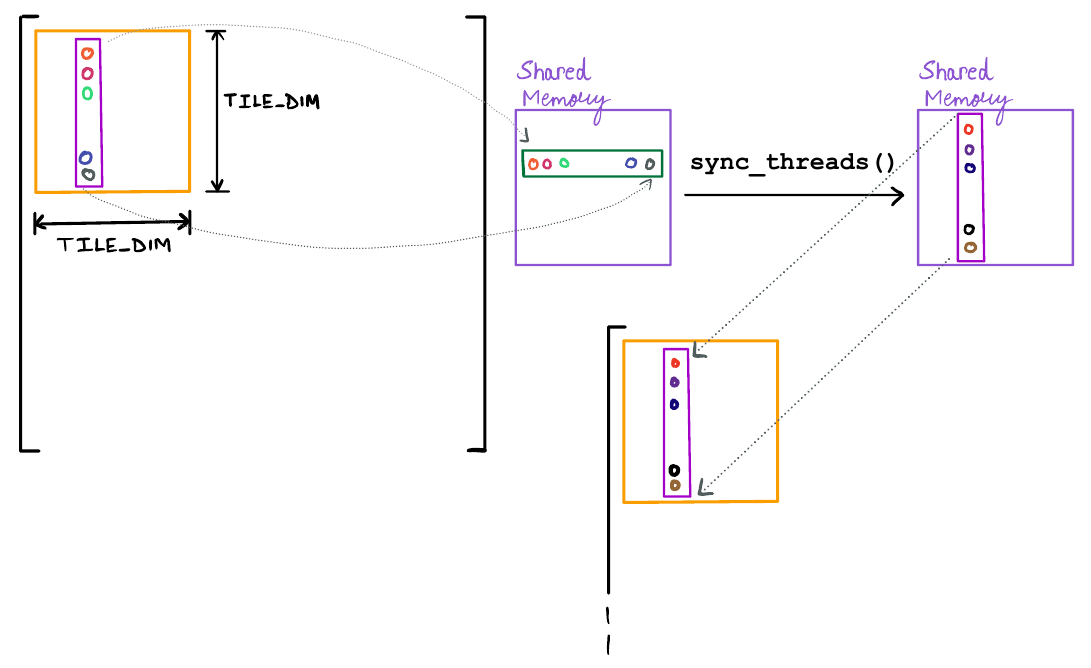
\includegraphics{./assets/coalesced_transpose.png}
\caption{Coalesced transpose}
\end{figure}



\begin{lstlisting}
(*@\HLJLk{function}@*) (*@\HLJLnf{gpu{\_}transpose{\_}kernel2}@*)(*@\HLJLp{(}@*)(*@\HLJLn{input}@*)(*@\HLJLp{,}@*) (*@\HLJLn{output}@*)(*@\HLJLp{)}@*)
    (*@\HLJLcs{{\#}}@*) (*@\HLJLcs{Declare}@*) (*@\HLJLcs{shared}@*) (*@\HLJLcs{memory}@*)
    (*@\HLJLn{shared}@*) (*@\HLJLoB{=}@*) (*@\HLJLnd{@cuStaticSharedMem}@*)(*@\HLJLp{(}@*)(*@\HLJLnf{eltype}@*)(*@\HLJLp{(}@*)(*@\HLJLn{input}@*)(*@\HLJLp{),}@*) (*@\HLJLp{(}@*)(*@\HLJLn{TILE{\_}DIM}@*)(*@\HLJLp{,}@*) (*@\HLJLn{TILE{\_}DIM}@*)(*@\HLJLp{))}@*)
    
    (*@\HLJLcs{{\#}}@*) (*@\HLJLcs{Modify}@*) (*@\HLJLcs{thread}@*) (*@\HLJLcs{index}@*) (*@\HLJLcs{so}@*) (*@\HLJLcs{threadIdx().x}@*) (*@\HLJLcs{dominates}@*) (*@\HLJLcs{the}@*) (*@\HLJLcs{column}@*)
    (*@\HLJLn{block{\_}index}@*) (*@\HLJLoB{=}@*) (*@\HLJLp{((}@*)(*@\HLJLnf{blockIdx}@*)(*@\HLJLp{()}@*)(*@\HLJLoB{.}@*)(*@\HLJLn{y}@*)(*@\HLJLp{,}@*) (*@\HLJLnf{blockIdx}@*)(*@\HLJLp{()}@*)(*@\HLJLoB{.}@*)(*@\HLJLn{x}@*)(*@\HLJLp{)}@*) (*@\HLJLoB{.-}@*) (*@\HLJLni{1}@*)(*@\HLJLp{)}@*) (*@\HLJLoB{.*}@*) (*@\HLJLn{TILE{\_}DIM}@*)
    
    (*@\HLJLk{for}@*) (*@\HLJLn{i}@*) (*@\HLJLkp{in}@*) (*@\HLJLni{1}@*)(*@\HLJLoB{:}@*)(*@\HLJLni{4}@*)
        (*@\HLJLn{thread{\_}index}@*) (*@\HLJLoB{=}@*) (*@\HLJLp{(}@*)(*@\HLJLnf{threadIdx}@*)(*@\HLJLp{()}@*)(*@\HLJLoB{.}@*)(*@\HLJLn{x}@*)(*@\HLJLp{,}@*) (*@\HLJLnf{threadIdx}@*)(*@\HLJLp{()}@*)(*@\HLJLoB{.}@*)(*@\HLJLn{y}@*) (*@\HLJLoB{+}@*) (*@\HLJLp{(}@*)(*@\HLJLn{i}@*) (*@\HLJLoB{-}@*) (*@\HLJLni{1}@*)(*@\HLJLp{)}@*)(*@\HLJLoB{*}@*)(*@\HLJLni{8}@*)(*@\HLJLp{)}@*)
        (*@\HLJLn{index}@*) (*@\HLJLoB{=}@*) (*@\HLJLnf{CartesianIndex}@*)(*@\HLJLp{(}@*)(*@\HLJLn{block{\_}index}@*) (*@\HLJLoB{.+}@*) (*@\HLJLn{thread{\_}index}@*)(*@\HLJLp{)}@*)

        (*@\HLJLp{(}@*)(*@\HLJLn{index}@*)(*@\HLJLp{[}@*)(*@\HLJLni{1}@*)(*@\HLJLp{]}@*) (*@\HLJLoB{>}@*) (*@\HLJLnf{size}@*)(*@\HLJLp{(}@*)(*@\HLJLn{input}@*)(*@\HLJLp{,}@*) (*@\HLJLni{1}@*)(*@\HLJLp{)}@*) (*@\HLJLoB{||}@*) (*@\HLJLn{index}@*)(*@\HLJLp{[}@*)(*@\HLJLni{2}@*)(*@\HLJLp{]}@*) (*@\HLJLoB{>}@*) (*@\HLJLnf{size}@*)(*@\HLJLp{(}@*)(*@\HLJLn{input}@*)(*@\HLJLp{,}@*) (*@\HLJLni{2}@*)(*@\HLJLp{))}@*) (*@\HLJLoB{{\&}{\&}}@*) (*@\HLJLk{continue}@*)
        (*@\HLJLnd{@inbounds}@*) (*@\HLJLn{shared}@*)(*@\HLJLp{[}@*)(*@\HLJLn{thread{\_}index}@*)(*@\HLJLp{[}@*)(*@\HLJLni{2}@*)(*@\HLJLp{],}@*) (*@\HLJLn{thread{\_}index}@*)(*@\HLJLp{[}@*)(*@\HLJLni{1}@*)(*@\HLJLp{]]}@*) (*@\HLJLoB{=}@*) (*@\HLJLn{input}@*)(*@\HLJLp{[}@*)(*@\HLJLn{index}@*)(*@\HLJLp{]}@*)
    (*@\HLJLk{end}@*)
    
    (*@\HLJLcs{{\#}}@*) (*@\HLJLcs{Barrier}@*) (*@\HLJLcs{to}@*) (*@\HLJLcs{ensure}@*) (*@\HLJLcs{all}@*) (*@\HLJLcs{threads}@*) (*@\HLJLcs{have}@*) (*@\HLJLcs{completed}@*) (*@\HLJLcs{writing}@*) (*@\HLJLcs{to}@*) (*@\HLJLcs{shared}@*) (*@\HLJLcs{memory}@*)
    (*@\HLJLnf{sync{\_}threads}@*)(*@\HLJLp{()}@*)
    
    (*@\HLJLcs{{\#}}@*) (*@\HLJLcs{swap}@*) (*@\HLJLcs{tile}@*) (*@\HLJLcs{index}@*)
    (*@\HLJLn{block{\_}index}@*) (*@\HLJLoB{=}@*) (*@\HLJLp{((}@*)(*@\HLJLnf{blockIdx}@*)(*@\HLJLp{()}@*)(*@\HLJLoB{.}@*)(*@\HLJLn{x}@*)(*@\HLJLp{,}@*) (*@\HLJLnf{blockIdx}@*)(*@\HLJLp{()}@*)(*@\HLJLoB{.}@*)(*@\HLJLn{y}@*)(*@\HLJLp{)}@*) (*@\HLJLoB{.-}@*) (*@\HLJLni{1}@*)(*@\HLJLp{)}@*) (*@\HLJLoB{.*}@*) (*@\HLJLn{TILE{\_}DIM}@*)
    
    (*@\HLJLk{for}@*) (*@\HLJLn{i}@*) (*@\HLJLkp{in}@*) (*@\HLJLni{1}@*)(*@\HLJLoB{:}@*)(*@\HLJLni{4}@*) 
        (*@\HLJLn{thread{\_}index}@*) (*@\HLJLoB{=}@*) (*@\HLJLp{(}@*)(*@\HLJLnf{threadIdx}@*)(*@\HLJLp{()}@*)(*@\HLJLoB{.}@*)(*@\HLJLn{x}@*)(*@\HLJLp{,}@*) (*@\HLJLnf{threadIdx}@*)(*@\HLJLp{()}@*)(*@\HLJLoB{.}@*)(*@\HLJLn{y}@*) (*@\HLJLoB{+}@*) (*@\HLJLp{(}@*)(*@\HLJLn{i}@*) (*@\HLJLoB{-}@*) (*@\HLJLni{1}@*)(*@\HLJLp{)}@*)(*@\HLJLoB{*}@*)(*@\HLJLni{8}@*)(*@\HLJLp{)}@*)
        (*@\HLJLn{index}@*) (*@\HLJLoB{=}@*) (*@\HLJLnf{CartesianIndex}@*)(*@\HLJLp{(}@*)(*@\HLJLn{block{\_}index}@*) (*@\HLJLoB{.+}@*) (*@\HLJLn{thread{\_}index}@*)(*@\HLJLp{)}@*)
        
        (*@\HLJLp{(}@*)(*@\HLJLn{index}@*)(*@\HLJLp{[}@*)(*@\HLJLni{1}@*)(*@\HLJLp{]}@*) (*@\HLJLoB{>}@*) (*@\HLJLnf{size}@*)(*@\HLJLp{(}@*)(*@\HLJLn{output}@*)(*@\HLJLp{,}@*) (*@\HLJLni{1}@*)(*@\HLJLp{)}@*) (*@\HLJLoB{||}@*) (*@\HLJLn{index}@*)(*@\HLJLp{[}@*)(*@\HLJLni{2}@*)(*@\HLJLp{]}@*) (*@\HLJLoB{>}@*) (*@\HLJLnf{size}@*)(*@\HLJLp{(}@*)(*@\HLJLn{output}@*)(*@\HLJLp{,}@*) (*@\HLJLni{2}@*)(*@\HLJLp{))}@*) (*@\HLJLoB{{\&}{\&}}@*) (*@\HLJLk{continue}@*)
        (*@\HLJLnd{@inbounds}@*) (*@\HLJLn{output}@*)(*@\HLJLp{[}@*)(*@\HLJLn{index}@*)(*@\HLJLp{]}@*) (*@\HLJLoB{=}@*) (*@\HLJLn{shared}@*)(*@\HLJLp{[}@*)(*@\HLJLn{thread{\_}index}@*)(*@\HLJLoB{...}@*)(*@\HLJLp{]}@*)
    (*@\HLJLk{end}@*)
    (*@\HLJLk{return}@*)
(*@\HLJLk{end}@*)

(*@\HLJLk{function}@*) (*@\HLJLnf{gpu{\_}transpose{\_}shmem}@*)(*@\HLJLp{(}@*)(*@\HLJLn{input}@*)(*@\HLJLp{,}@*) (*@\HLJLn{output}@*) (*@\HLJLoB{=}@*) (*@\HLJLnf{similar}@*)(*@\HLJLp{(}@*)(*@\HLJLn{input}@*)(*@\HLJLp{,}@*) (*@\HLJLp{(}@*)(*@\HLJLnf{size}@*)(*@\HLJLp{(}@*)(*@\HLJLn{input}@*)(*@\HLJLp{,}@*) (*@\HLJLni{2}@*)(*@\HLJLp{),}@*) (*@\HLJLnf{size}@*)(*@\HLJLp{(}@*)(*@\HLJLn{input}@*)(*@\HLJLp{,}@*) (*@\HLJLni{1}@*)(*@\HLJLp{))))}@*)
    (*@\HLJLn{threads}@*) (*@\HLJLoB{=}@*) (*@\HLJLp{(}@*)(*@\HLJLni{32}@*)(*@\HLJLp{,}@*) (*@\HLJLni{8}@*)(*@\HLJLp{)}@*)
    (*@\HLJLn{blocks}@*) (*@\HLJLoB{=}@*) (*@\HLJLn{cld}@*)(*@\HLJLoB{.}@*)(*@\HLJLp{(}@*)(*@\HLJLnf{size}@*)(*@\HLJLp{(}@*)(*@\HLJLn{input}@*)(*@\HLJLp{),}@*) (*@\HLJLp{(}@*)(*@\HLJLni{32}@*)(*@\HLJLp{,}@*) (*@\HLJLni{32}@*)(*@\HLJLp{))}@*)
    (*@\HLJLnd{@cuda}@*) (*@\HLJLn{blocks}@*)(*@\HLJLoB{=}@*)(*@\HLJLn{blocks}@*) (*@\HLJLn{threads}@*)(*@\HLJLoB{=}@*)(*@\HLJLn{threads}@*) (*@\HLJLnf{gpu{\_}transpose{\_}kernel2}@*)(*@\HLJLp{(}@*)(*@\HLJLn{input}@*)(*@\HLJLp{,}@*) (*@\HLJLn{output}@*)(*@\HLJLp{)}@*)
    (*@\HLJLn{output}@*)
(*@\HLJLk{end}@*)
\end{lstlisting}

\begin{lstlisting}
gpu(*@{{\_}}@*)transpose(*@{{\_}}@*)shmem (generic function with 2 methods)
\end{lstlisting}


\begin{lstlisting}
(*@\HLJLn{A}@*) (*@\HLJLoB{=}@*) (*@\HLJLnf{CuArray}@*)(*@\HLJLp{(}@*)(*@\HLJLnf{reshape}@*)(*@\HLJLp{(}@*)(*@\HLJLnfB{1f0}@*)(*@\HLJLoB{:}@*)(*@\HLJLni{1089}@*)(*@\HLJLp{,}@*) (*@\HLJLp{(}@*)(*@\HLJLni{33}@*)(*@\HLJLp{,}@*) (*@\HLJLni{33}@*)(*@\HLJLp{)))}@*)
(*@\HLJLn{B}@*) (*@\HLJLoB{=}@*) (*@\HLJLnf{similar}@*)(*@\HLJLp{(}@*)(*@\HLJLn{A}@*)(*@\HLJLp{)}@*)
(*@\HLJLnf{gpu{\_}transpose{\_}shmem}@*)(*@\HLJLp{(}@*)(*@\HLJLn{A}@*)(*@\HLJLp{,}@*) (*@\HLJLn{B}@*)(*@\HLJLp{)}@*)
\end{lstlisting}

\begin{lstlisting}
33(*@\ensuremath{\times}@*)33 CUDA.CuArray(*@{{\{}}@*)Float32,2(*@{{\}}}@*):
    1.0     2.0     3.0     4.0     5.0  (*@\ensuremath{\ldots}@*)    30.0    31.0    32.0    33.0
   34.0    35.0    36.0    37.0    38.0       63.0    64.0    65.0    66.0
   67.0    68.0    69.0    70.0    71.0       96.0    97.0    98.0    99.0
  100.0   101.0   102.0   103.0   104.0      129.0   130.0   131.0   132.0
  133.0   134.0   135.0   136.0   137.0      162.0   163.0   164.0   165.0
  166.0   167.0   168.0   169.0   170.0  (*@\ensuremath{\ldots}@*)   195.0   196.0   197.0   198.0
  199.0   200.0   201.0   202.0   203.0      228.0   229.0   230.0   231.0
  232.0   233.0   234.0   235.0   236.0      261.0   262.0   263.0   264.0
  265.0   266.0   267.0   268.0   269.0      294.0   295.0   296.0   297.0
  298.0   299.0   300.0   301.0   302.0      327.0   328.0   329.0   330.0
    (*@\ensuremath{\vdots}@*)                                    (*@\ensuremath{\ddots}@*)             (*@\ensuremath{\vdots}@*)            
  793.0   794.0   795.0   796.0   797.0      822.0   823.0   824.0   825.0
  826.0   827.0   828.0   829.0   830.0  (*@\ensuremath{\ldots}@*)   855.0   856.0   857.0   858.0
  859.0   860.0   861.0   862.0   863.0      888.0   889.0   890.0   891.0
  892.0   893.0   894.0   895.0   896.0      921.0   922.0   923.0   924.0
  925.0   926.0   927.0   928.0   929.0      954.0   955.0   956.0   957.0
  958.0   959.0   960.0   961.0   962.0      987.0   988.0   989.0   990.0
  991.0   992.0   993.0   994.0   995.0  (*@\ensuremath{\ldots}@*)  1020.0  1021.0  1022.0  1023.0
 1024.0  1025.0  1026.0  1027.0  1028.0     1053.0  1054.0  1055.0  1056.0
 1057.0  1058.0  1059.0  1060.0  1061.0     1086.0  1087.0  1088.0  1089.0
\end{lstlisting}


\begin{lstlisting}
(*@\HLJLn{A}@*) (*@\HLJLoB{=}@*) (*@\HLJLn{CUDA}@*)(*@\HLJLoB{.}@*)(*@\HLJLnf{rand}@*)(*@\HLJLp{(}@*)(*@\HLJLni{10000}@*)(*@\HLJLp{,}@*) (*@\HLJLni{10000}@*)(*@\HLJLp{)}@*)
(*@\HLJLn{B}@*) (*@\HLJLoB{=}@*) (*@\HLJLnf{similar}@*)(*@\HLJLp{(}@*)(*@\HLJLn{A}@*)(*@\HLJLp{)}@*)
(*@\HLJLnd{@benchmark}@*) (*@\HLJLn{CUDA}@*)(*@\HLJLoB{.}@*)(*@\HLJLnd{@sync}@*) (*@\HLJLnf{gpu{\_}transpose{\_}shmem}@*)(*@\HLJLp{(}@*)(*@\HLJLn{A}@*)(*@\HLJLp{,}@*) (*@\HLJLn{B}@*)(*@\HLJLp{)}@*)
\end{lstlisting}

\begin{lstlisting}
BenchmarkTools.Trial: 
  memory estimate:  320 bytes
  allocs estimate:  9
  --------------
  minimum time:     7.468 ms (0.00(*@{{\%}}@*) GC)
  median time:      7.676 ms (0.00(*@{{\%}}@*) GC)
  mean time:        7.794 ms (0.00(*@{{\%}}@*) GC)
  maximum time:     8.354 ms (0.00(*@{{\%}}@*) GC)
  --------------
  samples:          641
  evals/sample:     1
\end{lstlisting}


\begin{lstlisting}
(*@\HLJLnd{@benchmark}@*) (*@\HLJLn{CUDA}@*)(*@\HLJLoB{.}@*)(*@\HLJLnd{@sync}@*) (*@\HLJLn{B}@*) (*@\HLJLoB{.=}@*) (*@\HLJLn{A}@*)

(*@\HLJLcs{{\#}}@*) (*@\HLJLcs{TODO:}@*) (*@\HLJLcs{Doesn{\textquotesingle}t}@*) (*@\HLJLcs{look}@*) (*@\HLJLcs{like}@*) (*@\HLJLcs{an}@*) (*@\HLJLcs{inspiring}@*) (*@\HLJLcs{case.}@*) (*@\HLJLcs{We}@*) (*@\HLJLcs{should}@*) (*@\HLJLcs{investigate}@*) (*@\HLJLcs{why}@*) (*@\HLJLcs{the}@*) (*@\HLJLcs{broadcast}@*) (*@\HLJLcs{is}@*) (*@\HLJLcs{slower.}@*)
(*@\HLJLcs{{\#}}@*) (*@\HLJLcs{ofc}@*) (*@\HLJLcs{make}@*) (*@\HLJLcs{it}@*) (*@\HLJLcs{faster}@*) (*@\HLJLcs{so}@*) (*@\HLJLcs{that}@*) (*@\HLJLcs{there}@*) (*@\HLJLcs{is}@*) (*@\HLJLcs{an}@*) (*@\HLJLcs{inspiring}@*) (*@\HLJLcs{claim}@*) (*@\HLJLcs{of}@*) (*@\HLJLcs{how}@*) (*@\HLJLcs{there}@*) (*@\HLJLcs{is}@*) (*@\HLJLcs{more}@*) (*@\HLJLcs{room}@*) 
(*@\HLJLcs{{\#}}@*) (*@\HLJLcs{for}@*) (*@\HLJLcs{performance.}@*) (*@\HLJLcs{Making}@*) (*@\HLJLcs{"{}bank}@*) (*@\HLJLcs{conflicts"{}}@*) (*@\HLJLcs{the}@*) (*@\HLJLcs{next}@*) (*@\HLJLcs{natural}@*) (*@\HLJLcs{topic.}@*)
\end{lstlisting}

\begin{lstlisting}
BenchmarkTools.Trial: 
  memory estimate:  464 bytes
  allocs estimate:  13
  --------------
  minimum time:     7.483 ms (0.00(*@{{\%}}@*) GC)
  median time:      7.692 ms (0.00(*@{{\%}}@*) GC)
  mean time:        7.793 ms (0.00(*@{{\%}}@*) GC)
  maximum time:     8.372 ms (0.00(*@{{\%}}@*) GC)
  --------------
  samples:          641
  evals/sample:     1
\end{lstlisting}


\subsubsection{Shared Memory Bank conflicts}
Inside a , shared memory is divided into banks. Modern NVIDIA GPUs have 32 banks which have a 4-byte boundary. This means addresses 1-4 of shared memory are serviced by bank 1, addresses 5-8 are serviced by bank two and so on. When multiple threads access memory from the same bank then their requests are serialised.

Nsight compute gives statistics about shared memory usage. Running the profiler on \texttt{gpu\_transpose\_shmem} for an input of 33x33 of \texttt{Float32} we get:

\begin{figure}
\centering
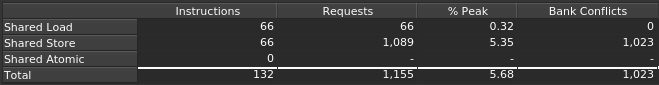
\includegraphics{./assets/shmem-conflicts.png}
\caption{shared-memory-conflicts}
\end{figure}


It reports zero conflicts during shared loads which makes sense during shared loads because we load column by column to write to output matrix.

The 1023 store conflicts can be explained as follows. When an entire column is read it is stored to a row. Consecutive elements in a row differ in address by \texttt{column\_length*sizeof(datatype)}. In 33 tile columns we write directly to a complete row where 32 elements are written hence there are 31 write conflicts. 33*31 = 1023

// DIAGRAM

The fix is quite simple, pad the column length in shared memory by 1. Now consecutive elements in a row will differ by 33 \% 32 = 1 hence no more bank conflicts.

i.e. \texttt{shared = @cuStaticSharedMem(eltype(input), (TILE\_DIM + 1, TILE\_DIM))}


\begin{lstlisting}
(*@\HLJLk{function}@*) (*@\HLJLnf{gpu{\_}transpose{\_}kernel3}@*)(*@\HLJLp{(}@*)(*@\HLJLn{input}@*)(*@\HLJLp{,}@*) (*@\HLJLn{output}@*)(*@\HLJLp{)}@*)
    (*@\HLJLcs{{\#}}@*) (*@\HLJLcs{Declare}@*) (*@\HLJLcs{shared}@*) (*@\HLJLcs{memory}@*)
    (*@\HLJLn{shared}@*) (*@\HLJLoB{=}@*) (*@\HLJLnd{@cuStaticSharedMem}@*)(*@\HLJLp{(}@*)(*@\HLJLnf{eltype}@*)(*@\HLJLp{(}@*)(*@\HLJLn{input}@*)(*@\HLJLp{),}@*) (*@\HLJLp{(}@*)(*@\HLJLn{TILE{\_}DIM}@*) (*@\HLJLoB{+}@*) (*@\HLJLni{1}@*)(*@\HLJLp{,}@*) (*@\HLJLn{TILE{\_}DIM}@*)(*@\HLJLp{))}@*)
    
    (*@\HLJLcs{{\#}}@*) (*@\HLJLcs{Modify}@*) (*@\HLJLcs{thread}@*) (*@\HLJLcs{index}@*) (*@\HLJLcs{so}@*) (*@\HLJLcs{threadIdx().x}@*) (*@\HLJLcs{dominates}@*) (*@\HLJLcs{the}@*) (*@\HLJLcs{column}@*)
    (*@\HLJLn{block{\_}index}@*) (*@\HLJLoB{=}@*) (*@\HLJLp{((}@*)(*@\HLJLnf{blockIdx}@*)(*@\HLJLp{()}@*)(*@\HLJLoB{.}@*)(*@\HLJLn{y}@*)(*@\HLJLp{,}@*) (*@\HLJLnf{blockIdx}@*)(*@\HLJLp{()}@*)(*@\HLJLoB{.}@*)(*@\HLJLn{x}@*)(*@\HLJLp{)}@*) (*@\HLJLoB{.-}@*) (*@\HLJLni{1}@*)(*@\HLJLp{)}@*) (*@\HLJLoB{.*}@*) (*@\HLJLn{TILE{\_}DIM}@*)
    
    (*@\HLJLk{for}@*) (*@\HLJLn{i}@*) (*@\HLJLkp{in}@*) (*@\HLJLni{1}@*)(*@\HLJLoB{:}@*)(*@\HLJLni{4}@*)
        (*@\HLJLn{thread{\_}index}@*) (*@\HLJLoB{=}@*) (*@\HLJLp{(}@*)(*@\HLJLnf{threadIdx}@*)(*@\HLJLp{()}@*)(*@\HLJLoB{.}@*)(*@\HLJLn{x}@*)(*@\HLJLp{,}@*) (*@\HLJLnf{threadIdx}@*)(*@\HLJLp{()}@*)(*@\HLJLoB{.}@*)(*@\HLJLn{y}@*) (*@\HLJLoB{+}@*) (*@\HLJLp{(}@*)(*@\HLJLn{i}@*) (*@\HLJLoB{-}@*) (*@\HLJLni{1}@*)(*@\HLJLp{)}@*)(*@\HLJLoB{*}@*)(*@\HLJLni{8}@*)(*@\HLJLp{)}@*)
        (*@\HLJLn{index}@*) (*@\HLJLoB{=}@*) (*@\HLJLnf{CartesianIndex}@*)(*@\HLJLp{(}@*)(*@\HLJLn{block{\_}index}@*) (*@\HLJLoB{.+}@*) (*@\HLJLn{thread{\_}index}@*)(*@\HLJLp{)}@*)

        (*@\HLJLp{(}@*)(*@\HLJLn{index}@*)(*@\HLJLp{[}@*)(*@\HLJLni{1}@*)(*@\HLJLp{]}@*) (*@\HLJLoB{>}@*) (*@\HLJLnf{size}@*)(*@\HLJLp{(}@*)(*@\HLJLn{input}@*)(*@\HLJLp{,}@*) (*@\HLJLni{1}@*)(*@\HLJLp{)}@*) (*@\HLJLoB{||}@*) (*@\HLJLn{index}@*)(*@\HLJLp{[}@*)(*@\HLJLni{2}@*)(*@\HLJLp{]}@*) (*@\HLJLoB{>}@*) (*@\HLJLnf{size}@*)(*@\HLJLp{(}@*)(*@\HLJLn{input}@*)(*@\HLJLp{,}@*) (*@\HLJLni{2}@*)(*@\HLJLp{))}@*) (*@\HLJLoB{{\&}{\&}}@*) (*@\HLJLk{continue}@*)
        (*@\HLJLnd{@inbounds}@*) (*@\HLJLn{shared}@*)(*@\HLJLp{[}@*)(*@\HLJLn{thread{\_}index}@*)(*@\HLJLp{[}@*)(*@\HLJLni{2}@*)(*@\HLJLp{],}@*) (*@\HLJLn{thread{\_}index}@*)(*@\HLJLp{[}@*)(*@\HLJLni{1}@*)(*@\HLJLp{]]}@*) (*@\HLJLoB{=}@*) (*@\HLJLn{input}@*)(*@\HLJLp{[}@*)(*@\HLJLn{index}@*)(*@\HLJLp{]}@*)
    (*@\HLJLk{end}@*)
    
    (*@\HLJLcs{{\#}}@*) (*@\HLJLcs{Barrier}@*) (*@\HLJLcs{to}@*) (*@\HLJLcs{ensure}@*) (*@\HLJLcs{all}@*) (*@\HLJLcs{threads}@*) (*@\HLJLcs{have}@*) (*@\HLJLcs{completed}@*) (*@\HLJLcs{writing}@*) (*@\HLJLcs{to}@*) (*@\HLJLcs{shared}@*) (*@\HLJLcs{memory}@*)
    (*@\HLJLnf{sync{\_}threads}@*)(*@\HLJLp{()}@*)
    
    (*@\HLJLcs{{\#}}@*) (*@\HLJLcs{swap}@*) (*@\HLJLcs{tile}@*) (*@\HLJLcs{index}@*)
    (*@\HLJLn{block{\_}index}@*) (*@\HLJLoB{=}@*) (*@\HLJLp{((}@*)(*@\HLJLnf{blockIdx}@*)(*@\HLJLp{()}@*)(*@\HLJLoB{.}@*)(*@\HLJLn{x}@*)(*@\HLJLp{,}@*) (*@\HLJLnf{blockIdx}@*)(*@\HLJLp{()}@*)(*@\HLJLoB{.}@*)(*@\HLJLn{y}@*)(*@\HLJLp{)}@*) (*@\HLJLoB{.-}@*) (*@\HLJLni{1}@*)(*@\HLJLp{)}@*) (*@\HLJLoB{.*}@*) (*@\HLJLn{TILE{\_}DIM}@*)
    
    (*@\HLJLk{for}@*) (*@\HLJLn{i}@*) (*@\HLJLkp{in}@*) (*@\HLJLni{1}@*)(*@\HLJLoB{:}@*)(*@\HLJLni{4}@*) 
        (*@\HLJLn{thread{\_}index}@*) (*@\HLJLoB{=}@*) (*@\HLJLp{(}@*)(*@\HLJLnf{threadIdx}@*)(*@\HLJLp{()}@*)(*@\HLJLoB{.}@*)(*@\HLJLn{x}@*)(*@\HLJLp{,}@*) (*@\HLJLnf{threadIdx}@*)(*@\HLJLp{()}@*)(*@\HLJLoB{.}@*)(*@\HLJLn{y}@*) (*@\HLJLoB{+}@*) (*@\HLJLp{(}@*)(*@\HLJLn{i}@*) (*@\HLJLoB{-}@*) (*@\HLJLni{1}@*)(*@\HLJLp{)}@*)(*@\HLJLoB{*}@*)(*@\HLJLni{8}@*)(*@\HLJLp{)}@*)
        (*@\HLJLn{index}@*) (*@\HLJLoB{=}@*) (*@\HLJLnf{CartesianIndex}@*)(*@\HLJLp{(}@*)(*@\HLJLn{block{\_}index}@*) (*@\HLJLoB{.+}@*) (*@\HLJLn{thread{\_}index}@*)(*@\HLJLp{)}@*)
        
        (*@\HLJLp{(}@*)(*@\HLJLn{index}@*)(*@\HLJLp{[}@*)(*@\HLJLni{1}@*)(*@\HLJLp{]}@*) (*@\HLJLoB{>}@*) (*@\HLJLnf{size}@*)(*@\HLJLp{(}@*)(*@\HLJLn{output}@*)(*@\HLJLp{,}@*) (*@\HLJLni{1}@*)(*@\HLJLp{)}@*) (*@\HLJLoB{||}@*) (*@\HLJLn{index}@*)(*@\HLJLp{[}@*)(*@\HLJLni{2}@*)(*@\HLJLp{]}@*) (*@\HLJLoB{>}@*) (*@\HLJLnf{size}@*)(*@\HLJLp{(}@*)(*@\HLJLn{output}@*)(*@\HLJLp{,}@*) (*@\HLJLni{2}@*)(*@\HLJLp{))}@*) (*@\HLJLoB{{\&}{\&}}@*) (*@\HLJLk{continue}@*)
        (*@\HLJLnd{@inbounds}@*) (*@\HLJLn{output}@*)(*@\HLJLp{[}@*)(*@\HLJLn{index}@*)(*@\HLJLp{]}@*) (*@\HLJLoB{=}@*) (*@\HLJLn{shared}@*)(*@\HLJLp{[}@*)(*@\HLJLn{thread{\_}index}@*)(*@\HLJLoB{...}@*)(*@\HLJLp{]}@*)
    (*@\HLJLk{end}@*)
    (*@\HLJLk{return}@*)
(*@\HLJLk{end}@*)

(*@\HLJLk{function}@*) (*@\HLJLnf{gpu{\_}transpose{\_}noconf}@*)(*@\HLJLp{(}@*)(*@\HLJLn{input}@*)(*@\HLJLp{,}@*) (*@\HLJLn{output}@*) (*@\HLJLoB{=}@*) (*@\HLJLnf{similar}@*)(*@\HLJLp{(}@*)(*@\HLJLn{input}@*)(*@\HLJLp{,}@*) (*@\HLJLp{(}@*)(*@\HLJLnf{size}@*)(*@\HLJLp{(}@*)(*@\HLJLn{input}@*)(*@\HLJLp{,}@*) (*@\HLJLni{2}@*)(*@\HLJLp{),}@*) (*@\HLJLnf{size}@*)(*@\HLJLp{(}@*)(*@\HLJLn{input}@*)(*@\HLJLp{,}@*) (*@\HLJLni{1}@*)(*@\HLJLp{))))}@*)
    (*@\HLJLn{threads}@*) (*@\HLJLoB{=}@*) (*@\HLJLp{(}@*)(*@\HLJLni{32}@*)(*@\HLJLp{,}@*) (*@\HLJLni{8}@*)(*@\HLJLp{)}@*)
    (*@\HLJLn{blocks}@*) (*@\HLJLoB{=}@*) (*@\HLJLn{cld}@*)(*@\HLJLoB{.}@*)(*@\HLJLp{(}@*)(*@\HLJLnf{size}@*)(*@\HLJLp{(}@*)(*@\HLJLn{input}@*)(*@\HLJLp{),}@*) (*@\HLJLp{(}@*)(*@\HLJLni{32}@*)(*@\HLJLp{,}@*) (*@\HLJLni{32}@*)(*@\HLJLp{))}@*)
    (*@\HLJLnd{@cuda}@*) (*@\HLJLn{blocks}@*)(*@\HLJLoB{=}@*)(*@\HLJLn{blocks}@*) (*@\HLJLn{threads}@*)(*@\HLJLoB{=}@*)(*@\HLJLn{threads}@*) (*@\HLJLnf{gpu{\_}transpose{\_}kernel3}@*)(*@\HLJLp{(}@*)(*@\HLJLn{input}@*)(*@\HLJLp{,}@*) (*@\HLJLn{output}@*)(*@\HLJLp{)}@*)
    (*@\HLJLn{output}@*)
(*@\HLJLk{end}@*)
\end{lstlisting}

\begin{lstlisting}
gpu(*@{{\_}}@*)transpose(*@{{\_}}@*)noconf (generic function with 2 methods)
\end{lstlisting}


\begin{lstlisting}
(*@\HLJLn{A}@*) (*@\HLJLoB{=}@*) (*@\HLJLn{CUDA}@*)(*@\HLJLoB{.}@*)(*@\HLJLnf{rand}@*)(*@\HLJLp{(}@*)(*@\HLJLni{10000}@*)(*@\HLJLp{,}@*) (*@\HLJLni{10000}@*)(*@\HLJLp{)}@*)
(*@\HLJLn{B}@*) (*@\HLJLoB{=}@*) (*@\HLJLnf{similar}@*)(*@\HLJLp{(}@*)(*@\HLJLn{A}@*)(*@\HLJLp{)}@*)
(*@\HLJLnd{@benchmark}@*) (*@\HLJLn{CUDA}@*)(*@\HLJLoB{.}@*)(*@\HLJLnd{@sync}@*) (*@\HLJLnf{gpu{\_}transpose{\_}noconf}@*)(*@\HLJLp{(}@*)(*@\HLJLn{A}@*)(*@\HLJLp{,}@*) (*@\HLJLn{B}@*)(*@\HLJLp{)}@*)
\end{lstlisting}

\begin{lstlisting}
BenchmarkTools.Trial: 
  memory estimate:  320 bytes
  allocs estimate:  9
  --------------
  minimum time:     6.049 ms (0.00(*@{{\%}}@*) GC)
  median time:      6.242 ms (0.00(*@{{\%}}@*) GC)
  mean time:        6.327 ms (0.00(*@{{\%}}@*) GC)
  maximum time:     6.992 ms (0.00(*@{{\%}}@*) GC)
  --------------
  samples:          789
  evals/sample:     1
\end{lstlisting}


\begin{lstlisting}
(*@\HLJLn{A}@*) (*@\HLJLoB{=}@*) (*@\HLJLn{CUDA}@*)(*@\HLJLoB{.}@*)(*@\HLJLnf{rand}@*)(*@\HLJLp{(}@*)(*@\HLJLni{10000}@*)(*@\HLJLp{,}@*) (*@\HLJLni{10000}@*)(*@\HLJLp{)}@*)
(*@\HLJLn{B}@*) (*@\HLJLoB{=}@*) (*@\HLJLnf{similar}@*)(*@\HLJLp{(}@*)(*@\HLJLn{A}@*)(*@\HLJLp{)}@*)
(*@\HLJLnd{@benchmark}@*) (*@\HLJLn{CUDA}@*)(*@\HLJLoB{.}@*)(*@\HLJLnd{@sync}@*) (*@\HLJLnf{gpu{\_}transpose{\_}shmem}@*)(*@\HLJLp{(}@*)(*@\HLJLn{A}@*)(*@\HLJLp{,}@*) (*@\HLJLn{B}@*)(*@\HLJLp{)}@*)
\end{lstlisting}

\begin{lstlisting}
BenchmarkTools.Trial: 
  memory estimate:  320 bytes
  allocs estimate:  9
  --------------
  minimum time:     7.489 ms (0.00(*@{{\%}}@*) GC)
  median time:      7.679 ms (0.00(*@{{\%}}@*) GC)
  mean time:        7.789 ms (0.00(*@{{\%}}@*) GC)
  maximum time:     8.367 ms (0.00(*@{{\%}}@*) GC)
  --------------
  samples:          642
  evals/sample:     1
\end{lstlisting}



\end{document}
